\documentclass{article}


\usepackage[backend=bibtex]{biblatex}
\usepackage{graphicx}
\usepackage{hyperref}
\usepackage{siunitx}
\usepackage[table]{xcolor}


\bibliography{report}
\title{Classifying rocks via 7810-dimensional spectroscopy}
\author{Miroslav Vitkov}


\begin{document}
\maketitle


\begin{abstract}
Several machine learning models in various C++ libraries are utilised\footnote{https://github.com/MiroslavVitkov/rocks}.
The most promising one is then tuned - kernel type, kernel parameters, data preprocessing.
The business application accuracy is theoretically derived from the per sample accuracy.
\end{abstract}


\section{Dataset}
Laser-induced breakdown spectroscopy\cite{libs_intro} involves turning some matter into plasma and observing it's radiant spectrum.
That is measured by a spectrometer and discretized into 7810 buckets of central frequency from  \SI{180}{\nano\metre} upward in steps of \SI{0.1}{\nano\metre}.
The spectrometer has an apparent peak in sensitivity around \SI{440}{\nano\metre} but important spectral lines are spread through the whole measurement range.
\par
The 7810 measured values for each spectrum represent the radiance\cite{radiance} of the plasma convoluted with the \textbf{unknown} impulse response of the measurement equipment.
\par
The dataset consists of 2710 datapoints all classified within 6 labels and 45 sublabels( measurement neighbourhoods ).
The reference number of the dataset is 190401.
The excitation laser wavelength is \SI{1064}{\nano\metre}.


\section{Noise}
Boiling plasma is not theoretically expected to absorb light of any wavelength.
The dataset violates this assumption!
\par
\begin{verbatim}
Dataset consists of 2710 files.
The global micro average intensity is 114.398.
The global count of negative values is 2442125, which is 0.115385 of all datapoints.
The mean of all negative values is -9.10135.
The most extreme negative value is -1042.48.
\end{verbatim}
\begin{itemize}
\item{One model of the noise is harmonics of the exciting laser.
This hypothesis fails due to it operating at \SI{1064}{\nano\metre}, which is not a multiple of the observed spikes' frequency.}
\item{Another model is Gaussian noise with $\mu=\SI{440}{\nano\metre}, \sigma=\SI{40}{\nano\metre}$.}
\item{Another model is uniform noise, multiplied by the impulse response of the measurement equipment.
Instrument IR can be recovered by averaging each frequency's mean value over all samples (i.e. stochastic multidimensional mean).}
\end{itemize}
\begin{figure}
\caption{Most extreme negative intensity}
\centering
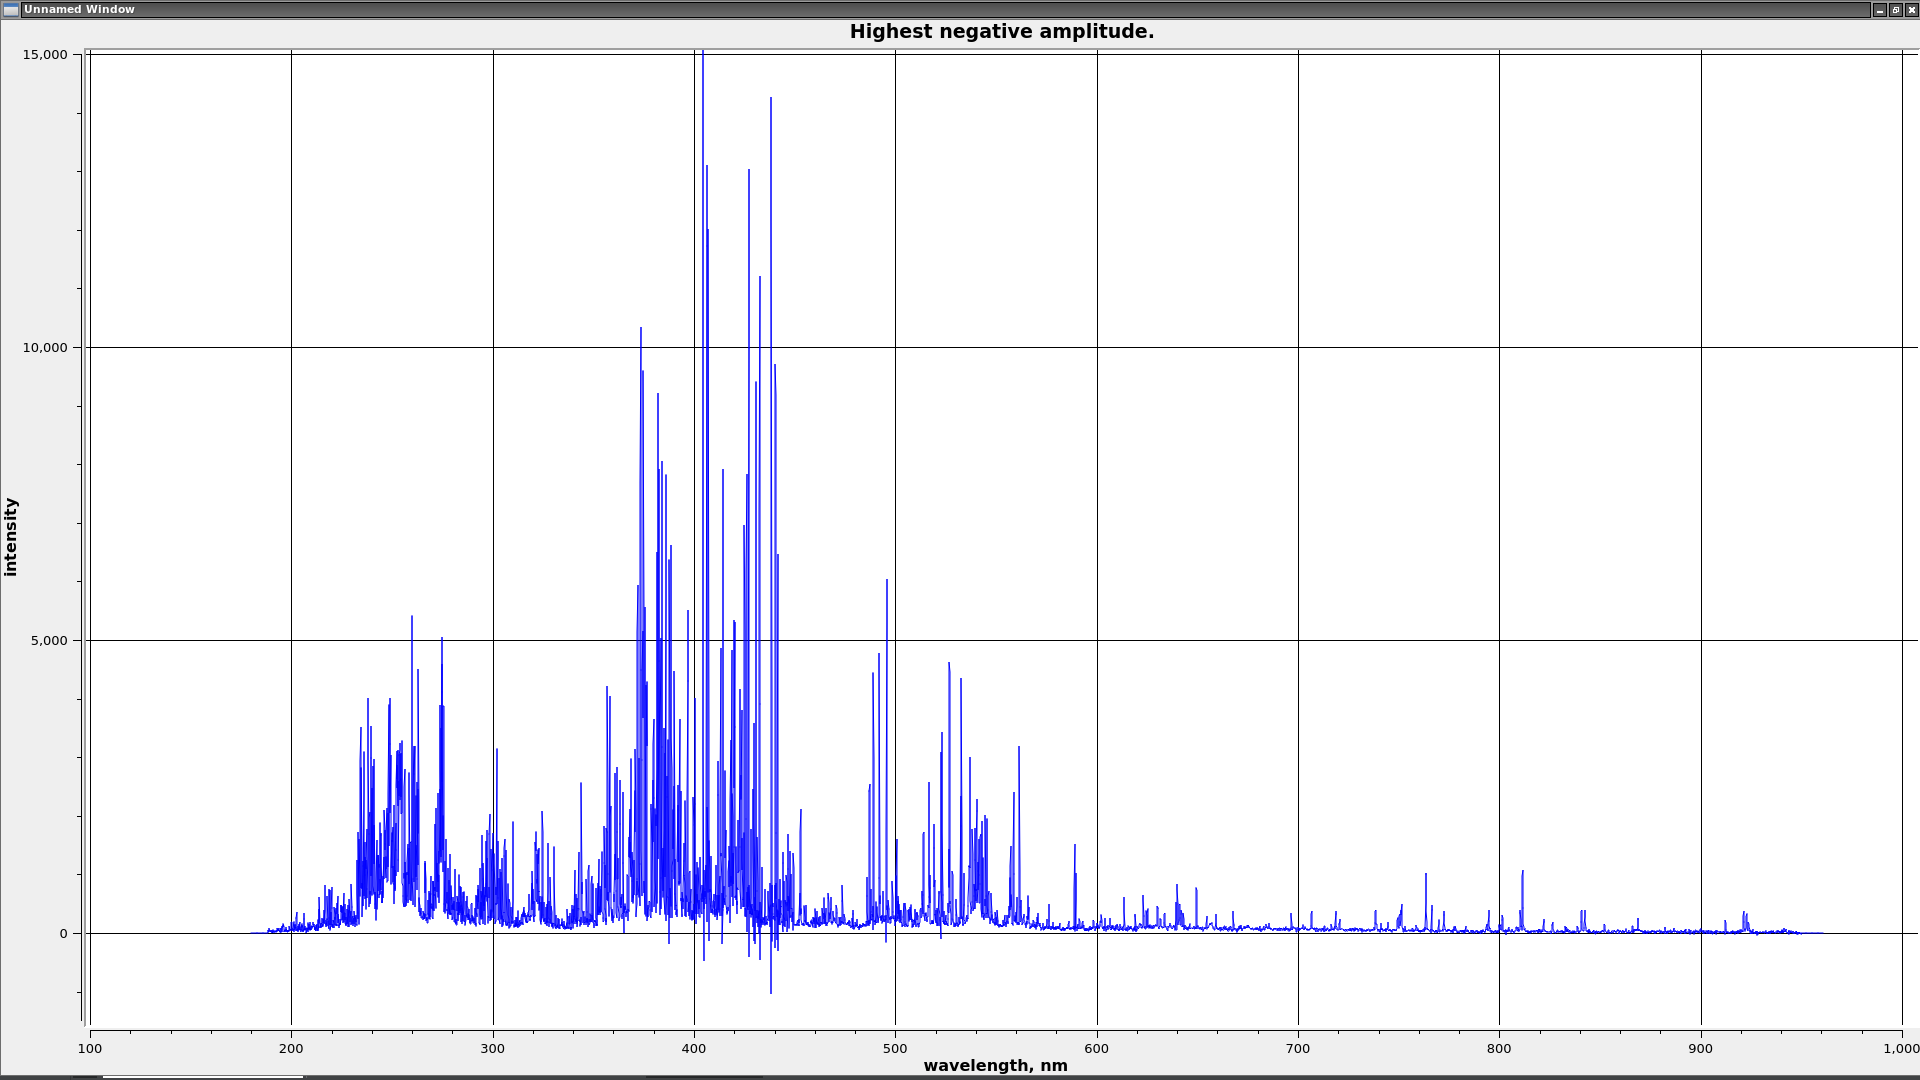
\includegraphics[width=1.25\textwidth]{img/negatives}
\end{figure}
Noise filtering has not been implemented.


\section{Dimensionality Reduction}
The number of features (7810) is larger than the dataset size(2711).
Thus better performance is expected from the classifiers after dimensionality reduction.

On the other hand, feature selection techniques should point to prominent spectral lines.
Those could be valuable to domain experts.


\subsection{Akaike information criterion}
Information gain was not used as prominent feature selector due to time constraints.


\subsection{Principal component analysis}
Plotting a few samples from 2 classes illustrates the data is not linearly separable.
The used SVM must be using a soft margin.
\\
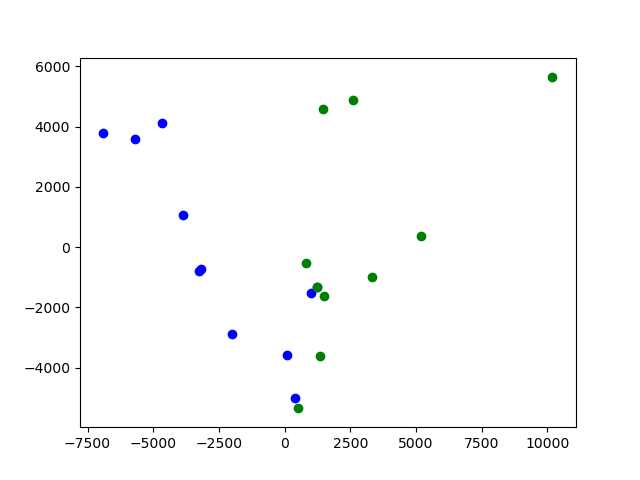
\includegraphics[width=0.9\textwidth]{img/pca}
\\
When attempting to classify only by the top 5 basis vectors, the SVM accuracy fell from 0.97 to 0.51.


\subsection{Linear discriminant analysis}
Like \textit{sklearn}'s LDA implementation, \textit{OpenCV}'s results in at most (num classes - 1) dimensional transformed space.
For the examined dataset \textit{d=5}.
The classification accuracy of the SVM dropped from 0.97 to 0.18.


\subsection{t-SNE}
For comparison, a t-distributed stochastic neighbour embedding should have been run.
But due to time constraints was not.


\section{Preprocessing}
\subsection{Normalization}
Normalization surprisingly worsened performance from 0.97 to 0.93.


\subsection{Logaritm}
Compressing the signal range worsened the accuracy from 0.97 to 0.77.


\section{Models}
The following algorithms were tried with default parameters from the corresponding libraries implementing them.
\\ \par
\rowcolors{1}{white}{lightgray}
\begin{tabular}{ c | c | c | c | c }
algorithm      & micro averaged accuracy & prediction time  & training time                    & computational model \\
random chance  & 0.16                    & \SI{0}{\second}  & \SI{0}{\second}                  & single thread \\
correlation    & 0.85                    & \SI{76}{\second} & \SI{0}{\second}                  & multi-threaded \\
SVM            & 0.97                    & \SI{0}{\second}  & \SI{3}{\minute} \SI{21}{\second} & multi-thread \\
neural network & 0.20                    & \SI{0}{\second}  & \SI{2}{\minute} \SI{7}{\second}  & GPU \\  % doesn't work anymore!! evil dlib!
random forest  & 0.17                    & \SI{21}{\second} & \SI{1}{\hour} \SI{49}{\minute}   & multi-threaded \\  % doesn't work! evil andres::trees
\end{tabular}


\subsection{Random Chance}
For sanity checking of the system, a random chance model was developed.
It looks only at the distribution of training labels and produces a similar stochastic distribution at prediction time.
An alternative would have been to always predict the most common class.
That would have improved repeatability between runs, but the generated distribution would have been too different than that of a predictive model.


\subsection{Correlation}
With such a small dataset, correlation is feasible.
It yields good results, but is not scalable.


\subsection{SVM}
A multiclass SVM is tested with a linear kernel because that is the only one dlib supports.

%maximum-margin classifier
%kernel trick
%hard/soft margin
%Radial basis function kernel
%http://webspace.ulbsibiu.ro/lucian.vintan/html/sci.pdf
%one vs one / one vs many
%curse of dimensionality
%https://stats.stackexchange.com/questions/77876/why-would-scaling-features-decrease-svm-performance?rq=1
%https://arxiv.org/pdf/0810.4752v1.pdf
%https://stats.stackexchange.com/questions/10423/number-of-features-vs-number-of-observations/10426#10426
%https://stats.stackexchange.com/a/10426/208261
%https://stats.stackexchange.com/questions/186184/does-dimensionality-curse-effect-some-models-more-than-others
%choice of regularization coefficient c
%choice of kernel
%choice of kernel parameters
% probabilistic classifier


\subsection{Neural Network}
A naive model with two hidden layers with relu activations performed extremely poorly.
It is unclear if this is due to programming errors or due to wrong architecture of the network.


\subsection{Random Forest}
An OpenMP-based random forest classifier took extremely long to train and yielded poor results.


\section{Measuring Accuracy}
Accuracy in the case of multiclass classification is not uniquely defined.
Those are the two approaches:
\begin{itemize}
\item{Micro average - record a True Positive and Total statistics among all classes. }
\item{Macro average - compute the accuracy for each class, then average those.}
\end{itemize}


\section{Tuning the model}
The SVM model performs well and runs quickly at prediction time.
This model is selected for parameter tuning.
However, the used implementation allows the use only linear kernels for multiclass SVMs (why)?
A grid search for the regularization coefficient c in the range [1e-5, 1e5] indicates said space is rather flat.

\begin{tabular}{ c | c }
c & accuracy  \\
1e-5 & 0.788652  \\
1e-4 & 0.780142  \\
1e-3 & 0.798582  \\
1e-2 & 0.794326  \\
1e-1 & 0.798582  \\
1e0 & 0.802837  \\
1e1 & 0.792908  \\
1e2 & 0.801418  \\
1e3 & 0.791489  \\
1e4 & 0.807092  \\
1e5 & 0.798582  \\
\end{tabular}

Also notice the drop in accuracy compared to the results reported in chapter 'Model'.
This is due to training on a smaller dataset, due to withholding the validation partition.
Naturally, both the training and validation partitions sets are used to train the final classifier.


\section{Implementation}
\subsection{Language}
C++ was chosen as the language of the implementation.


\subsection{Design}
The program uses the \textbf{Command} design pattern to fit different working modes into one executable.

The classifier models follow the Open/Close OOP principle.
They should have worked with either raw spectra or with preprocessed data, but that would have complicated the interface design.
Thus preprocessing techniques were tested in hardcoded SVMandX models.

To separate interface from implementation \textbf{pImpl} is used.
Not only do implementation details remain hidden, external includes also remain only in the .cpp file.

The \textbf{Factory} model::create() connects seamlessly with the command line parser module.

\subsection{Reproducibility}
Probably due to programming errors on our part, the PCA and SVM models produce slightly different results from run to run.
The presented results are averaged over several runs.

\subsection{Libraries}
\begin{itemize}
\item{dlib - a small mathematical library, used for correlation, neural networks, SVM.}
\item{Qwt - a native plotting library. It's main rival are the C++ bindings for pyplot.}
\item{OpenCV - used for PCA, because dlib's methods only work for binary classification out of the box.}
\end{itemize}

\subsection{Data structures}
Traditionally a dataframe is used to store and represent a dataset.
To the contrary we used a map from labels to a set of observations.
A function was provided for walking this structure.
Overall this setup performs well except when the shape of the dataframe needs to change.


\section{Implications}
Majority voting with n=60 samples and accuracy a=0.9828 yields overall expected error rate of
\begin{verbatim}
$ find . -name *.csv | wc -l
2710
$ calc "2710 / 45"
~60.22222
>>> import math
>>> # Probability of majority voting to fail:
>>> # ( 1 - 0.9828 ) ^ 30 + ( 1 - 0.9828 ) ^ 31 + ... + ( 1 - 0.9828 ) ^ 60
>>> # Let's take only the largest term.
>>> math.pow(( 1 - 0.9828 ),30)
1.163733153901975e-53
>>> # Let's assume one test per second.
>>> # The Mean Time Between Failures is the invese of the frequency of failures.
>>> 1 / 1.163733153901975e-53
8.593035238766027e+52  # seconds
>>> # Let's divide this by the age of the universe.
>>> 8.593035238766027e+52 / ( 31557600 * 13.8e9 )
1.973165617645385e+35
\end{verbatim}


\section{Conclusion}
\subsection{Sampling}
To keep the test environment close to the intended operation of the device, the following partitioning policy is adopted.
For each label, the first measured spot (with up to 64 measured spectra) is the test sample, the rest is training data.


\subsection{Experimental}
A large number of test points which are guaranteed to be of the same label is provided during real world operation.
This results in even a simple model like an SVM solving the problem practically perfectly.

\subsection{Language}
Customarily machine learning is done in Python.
Those are our observations over the suitability of C++ for such tasks.
\begin{itemize}
\item{Central repository - Python "comes with the batteries included".
                           Somewhat mitigating this, this project uses a plethora of libraries known to be open-source, with permissive license, easy to use, efficient.
                           The project thus can be used as a demo of C++ ML libraries.
}
\item{Type safety - due to the nature of matrix multiplication, the result is rarely in the same form as the input.
                    Thus new types need to be created between any two operations, making pipelining more tedious.
                    Overall little is gained by labelling lists of numbers which change their representation but preserve their meaning.}
\item{Plotting - plotting libraries for C++ are scarce, one of the most popular candidates being the bindings to matplotlib.}
\item{Dataframes - matrix calculations, consistency between test run results.}
\end{itemize}


\printbibliography


\end{document}
